\documentclass[xcolor=table,aspectratio=169]{beamer}

% General settings
\usetheme{Madrid}
\usepackage[T1]{fontenc}
\usepackage{graphicx}

\usepackage{xskak,chessboard}

% Remove navigation symbols
\beamertemplatenavigationsymbolsempty

% Fonts
\usepackage{helvet}
\setbeamerfont{normal text}{family=helvet}
\setbeamerfont{local structure}{family=helvet}

% Colors
\definecolor{kgrey}{HTML}{2b2828}
\setbeamercolor{frametitle}{bg=kgrey,fg=white}
\setbeamercolor{block title}{bg=kgrey,fg=white}

% Lists
\setbeamertemplate{enumerate items}[default]
\setbeamertemplate{itemize items}{\normalsize $\bullet$}
\setbeamercolor{description item}{fg=kgrey}
\setbeamercolor{enumerate item}{fg=kgrey}
\setbeamercolor{itemize item}{fg=kgrey}
\setbeamercolor{itemize subitem}{fg=kgrey}
\setbeamercolor{itemize subsubitem}{fg=kgrey}

% Templates
\setbeamertemplate{blocks}[default]
\setbeamertemplate{frametitle}{}
\setbeamertemplate{footline}{}
\usepackage{tcolorbox}
\tcbuselibrary{skins,hooks}
\tcbset{colframe=structure,fonttitle=\bfseries,beamer, clip upper, boxsep=0pt, sharp corners=all, no shadow, left skip=0pt, right skip=0pt, coltext=white}
\setbeamertemplate{title page}
{
  \leavevmode%
  \vbox{%
  \vspace{-1.6ex}%
  \noindent\begin{tcolorbox}[enhanced,watermark graphics=photo.png, width=\paperwidth, height=0.575\paperwidth, watermark zoom=1.25, grow to left by=0.035\paperwidth, frame hidden]

  \vspace{7.5em}
  \begin{center} 
  \huge
  \textbf{\inserttitle}

  \end{center}
  \end{tcolorbox}

  \vspace{-2em}
  \begin{tcolorbox}[width=\paperwidth, enhanced, colback=kgrey, grow to left by=0.035\paperwidth,]
  \begin{center}
  \footnotesize \bf \insertauthor\quad | \quad \insertdate    
  \end{center}
  \end{tcolorbox}
  }
}

\title{MARVEL Pub Quiz}
\author{Edward Linscott}
\date{17 Jan 2024}
\begin{document}
\frame{\titlepage}
\begin{frame}
   The format:
   \begin{itemize}[<+(1)->]
      \item five regular rounds
      \begin{itemize}
         \item eight questions each, which we will go through together
         \item questions within each round are linked by some common thread
      \end{itemize}
      \item picture and puzzle rounds
      \begin{itemize}
         \item for you to complete in your spare time
         \item examples to follow
      \end{itemize}
   \end{itemize}

   \onslide<8->{The etiquette:}
   \begin{itemize}[<+(1)->]
      \item if you need something clarified, just ask!
      \item at the end of each round I can repeat previous questions upon request, so don't worry if you've forgotten what a previous question was
      \item the quizmaster is \emph{always} right
   \end{itemize}
\end{frame}

\begin{frame}
   Example picture

   \begin{center}
      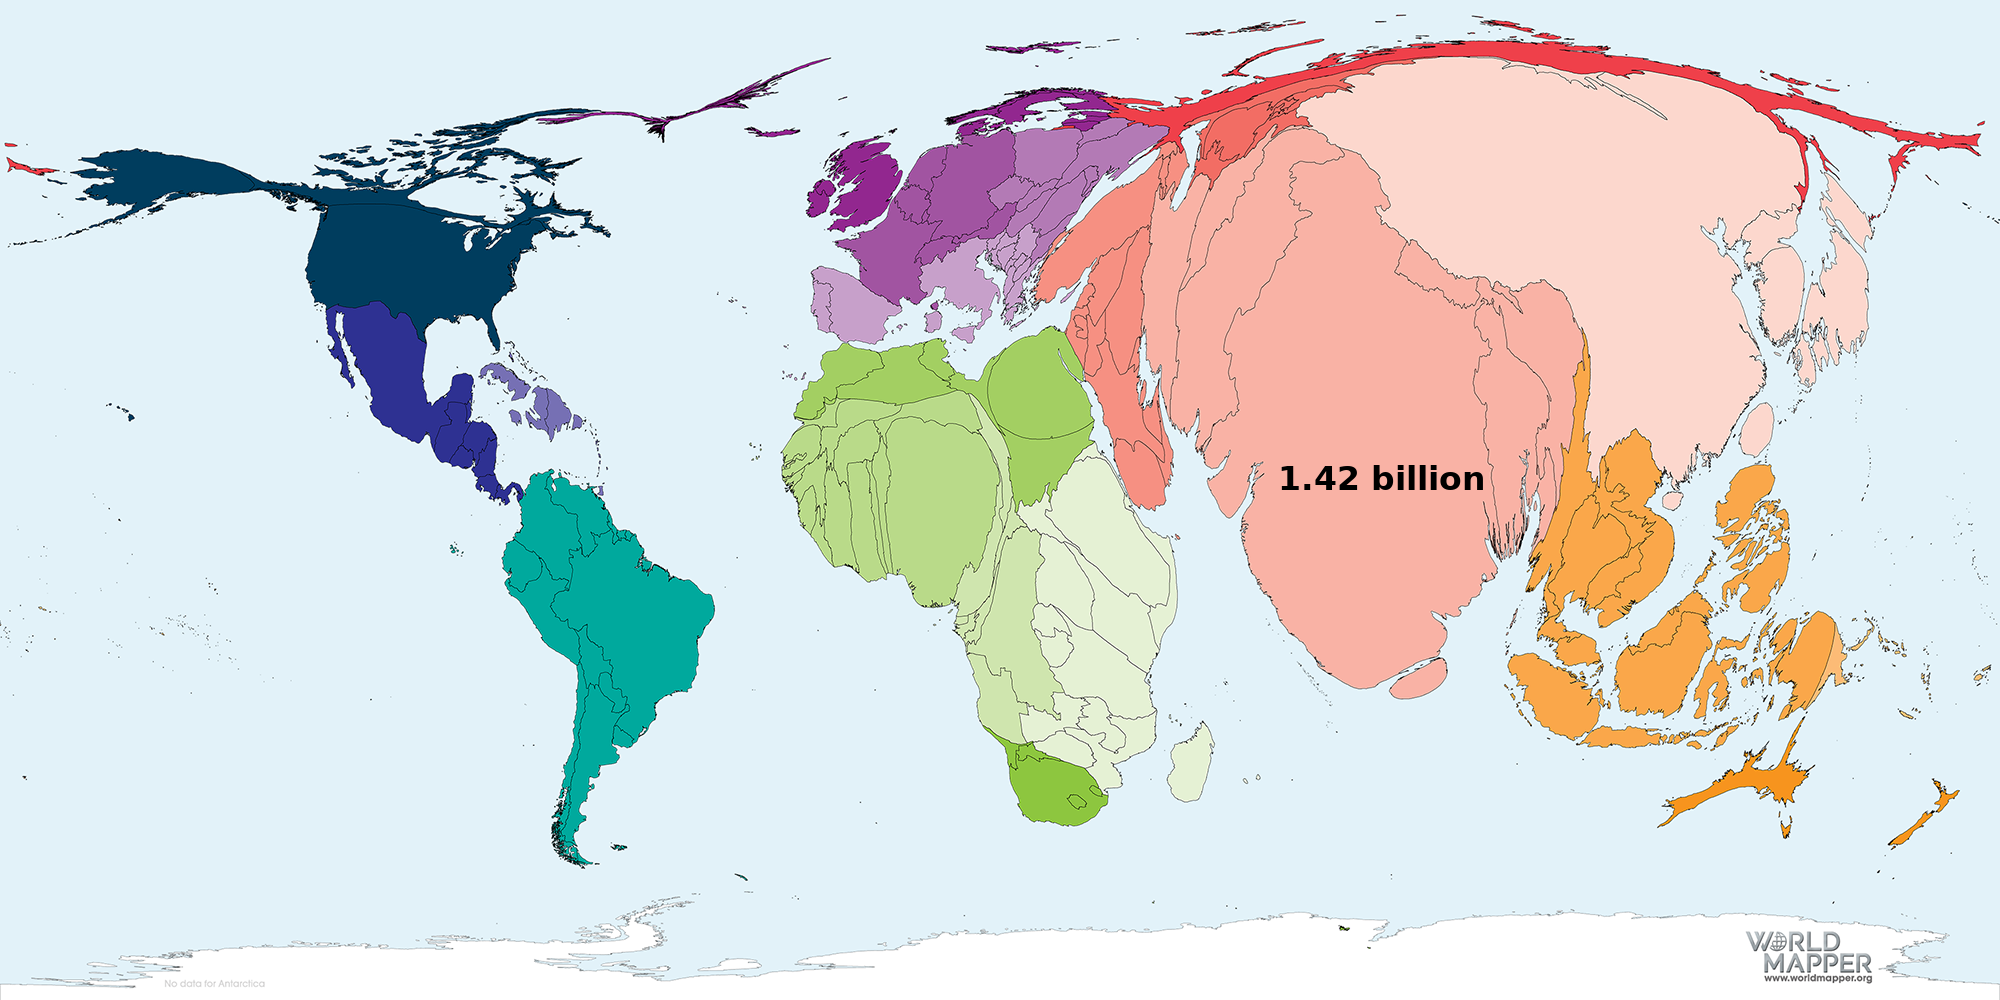
\includegraphics[width=0.6\paperwidth]{maps/population.png}

      \onslide<2->{population}
   \end{center}
\end{frame}

\begin{frame}
    \large
    Example puzzle 1. What links
          \begin{center}
                  magic, hugo, alfa, california
          \end{center}
   \onslide<2->{\textit{They all combine with a word from the NATO alphabet: Magic Mike, Victor Hugo, Alfa Romeo, and Hotel California}}
\end{frame}

\begin{frame}
   \large
   Example puzzle 2. What links
   \begin{center}
      \begin{minipage}{0.6\textwidth}
          \textit{%
              pe (skateboarding) \onslide<3->{= half-pi\textbf{pe}} \\
              thon (athletics) \onslide<4->{= half mara\textbf{thon}} \\
              son (wrestling) \onslide<5->{= half nel\textbf{son}} \\
              ley (tennis) \onslide<6->{= half-vol\textbf{ley}}}%
      \end{minipage}
   \end{center}

   \onslide<2->{Halves}%

\end{frame}

\begin{frame}
\begin{center}
\Huge
Round 1: Switzerland
\end{center}
\end{frame}
\begin{frame}
\begin{center}
\Large
1. Skiing is a very, very, old activity. The earliest evidence of skiing comes from which country?
\end{center}
\end{frame}
\begin{frame}
\begin{center}
\Large
2. In "A Big Day Out", why do Wallace and Gromit go to the moon?
\end{center}
\end{frame}
\begin{frame}
\begin{center}
\Large
3. Which 2000 romance saw Johnny Depp star as the love interest of Juliette Binoche?
\end{center}
\end{frame}
\begin{frame}
\begin{center}
\Large
4. What object has a face, a crown, and a lug?
\end{center}
\end{frame}
\begin{frame}
\begin{center}
\Large
5. Which federation was founded in 1904 by representatives from France, Belgium, Denmark, Spain, Sweden and the Netherlands?
\end{center}
\end{frame}
\begin{frame}
\begin{center}
\Large
6. This is an emblem of which organisation?
\\
\vspace{0.5em}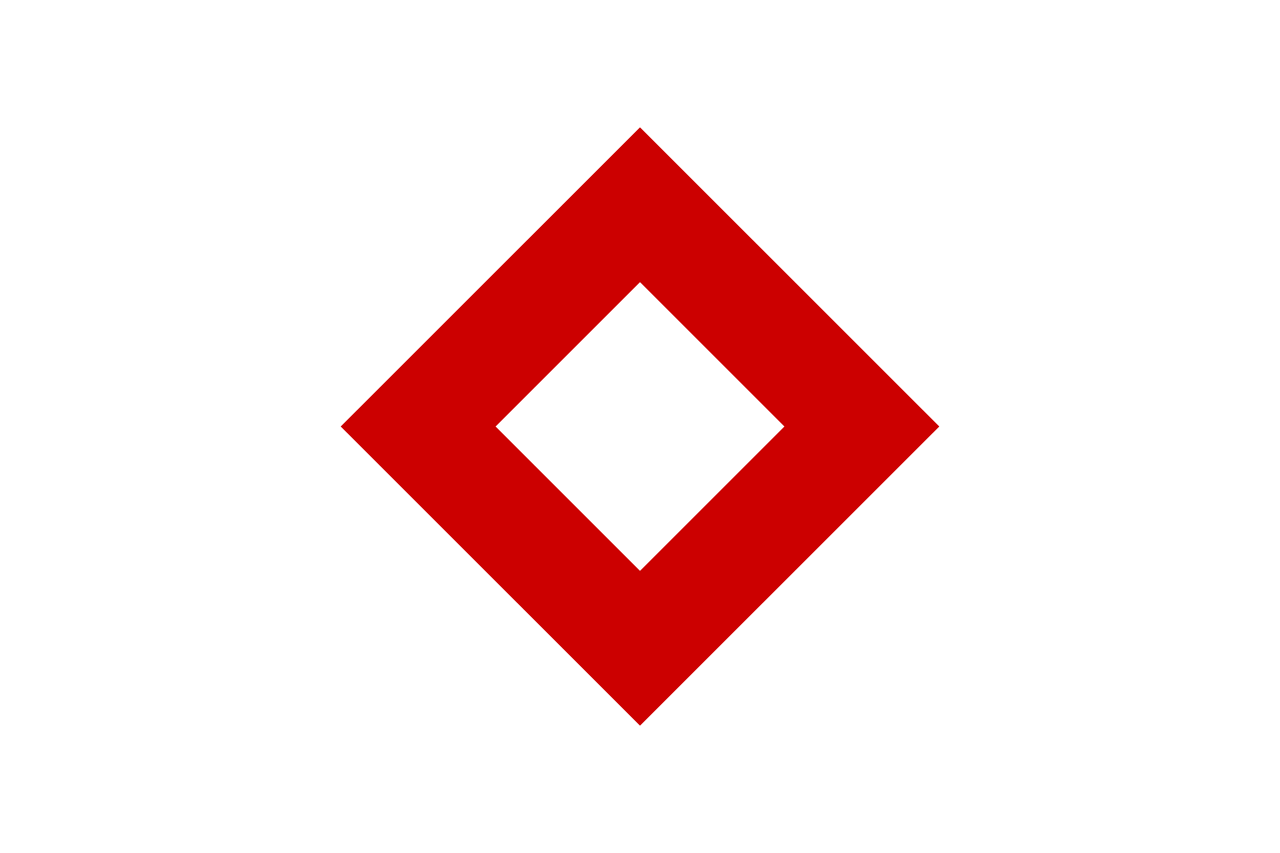
\includegraphics[height=0.6\paperheight]{images/red_crystal.png}
\end{center}
\end{frame}
\begin{frame}
\begin{center}
\Large
7. Which of the following is NOT a Swiss tradition:
\begin{itemize}
\item cow-vs-cow fighting
\item burning a snowman
\item cow parades as they descend from the mountains
\item throwing and twirling flags
\item gathering to ski on the summer solstice
\item men dressing up as bushes
\item a sport that's a cross between golf and baseball
\item a turnip parade
\item a parade at 4 a.m.
\end{itemize}

\end{center}
\end{frame}
\begin{frame}
\begin{center}
\Huge
Answers
\end{center}
\end{frame}
\begin{frame}
\begin{center}
\Large
1. Skiing is a very, very, old activity. The earliest evidence of skiing comes from which country?
\\
\onslide<2->{\vspace{1em}\textit{Russia}}
\end{center}
\end{frame}
\begin{frame}
\begin{center}
\Large
2. In "A Big Day Out", why do Wallace and Gromit go to the moon?
\\
\onslide<2->{\vspace{1em}\textit{to get some cheese}}
\end{center}
\end{frame}
\begin{frame}
\begin{center}
\Large
3. Which 2000 romance saw Johnny Depp star as the love interest of Juliette Binoche?
\\
\onslide<2->{\vspace{1em}\textit{Chocolat}}
\end{center}
\end{frame}
\begin{frame}
\begin{center}
\Large
4. What object has a face, a crown, and a lug?
\\
\onslide<2->{\vspace{1em}\textit{A watch}}
\end{center}
\end{frame}
\begin{frame}
\begin{center}
\Large
5. Which federation was founded in 1904 by representatives from France, Belgium, Denmark, Spain, Sweden and the Netherlands?
\\
\onslide<2->{\vspace{1em}\textit{FIFA}}
\end{center}
\end{frame}
\begin{frame}
\begin{center}
\Large
6. This is an emblem of which organisation?
\\
\only<1>{\vspace{0.5em}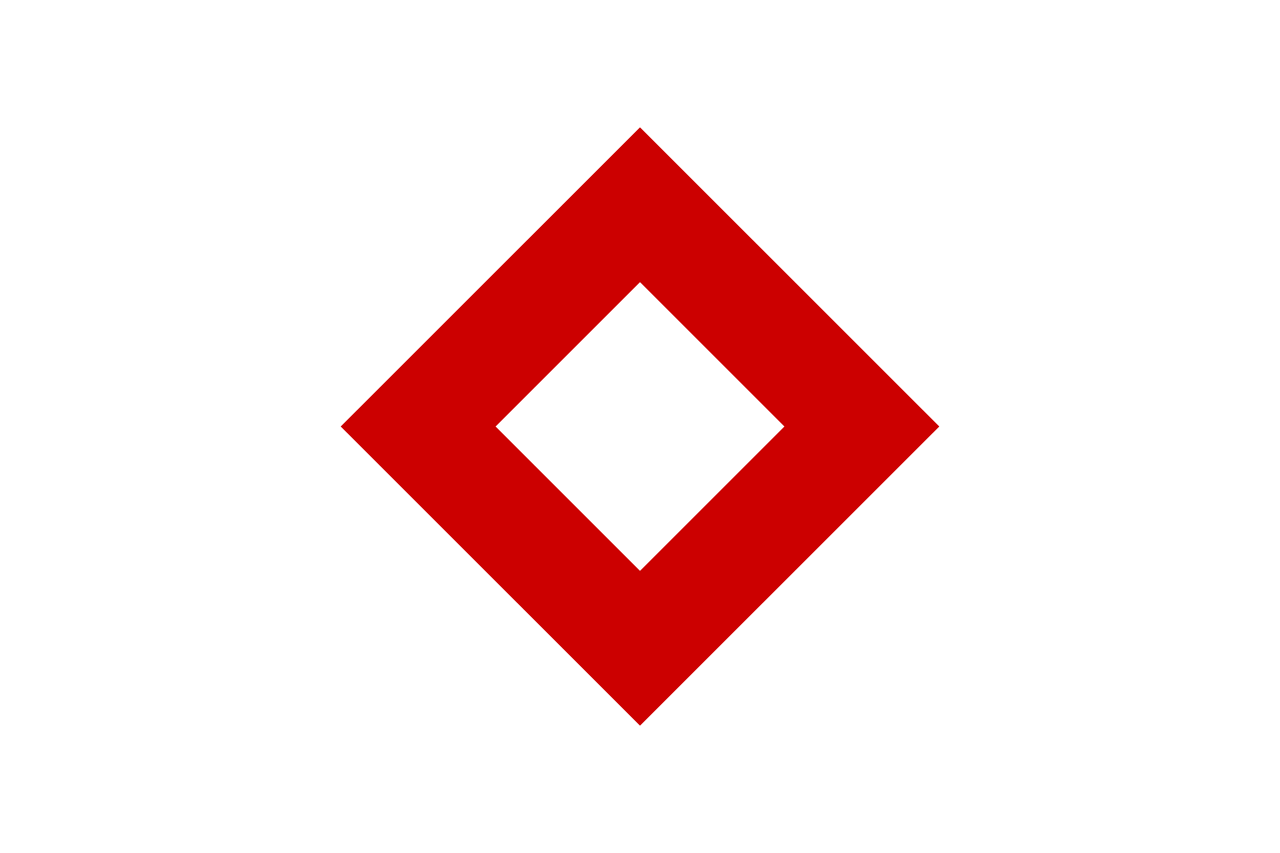
\includegraphics[height=0.6\paperheight]{images/red_crystal.png}}
\only<2>{\vspace{0.5em}
\includegraphics[height=0.3\paperheight]{images/red_cross_cresent_crystal.png}}
\\
\onslide<2->{\vspace{1em}\textit{The Red Cross}}
\end{center}
\end{frame}
\begin{frame}
\begin{center}
\Large
7. Which of the following is NOT a Swiss tradition:
\begin{itemize}
\item cow-vs-cow fighting
\item burning a snowman
\item cow parades as they descend from the mountains
\item throwing and twirling flags
\item gathering to ski on the summer solstice
\item men dressing up as bushes
\item a sport that's a cross between golf and baseball
\item a turnip parade
\item a parade at 4 a.m.
\end{itemize}

\onslide<2->{\vspace{1em}\textit{skiing on the summer solstice}}
\end{center}
\end{frame}
\begin{frame}
\begin{center}
\Huge
Round 2: ``Marvel''
\end{center}
\end{frame}
\begin{frame}
\begin{center}
\Large
1. Of all the films in the MARVEL cinematic universe, which has the highest rating on Rotten Tomatoes
\end{center}
\end{frame}
\begin{frame}
\begin{center}
\Large
2. Something about wonders - The Great Pyramids of Giza, Great Wall of China, The Grand Canyon, The Grand Tetons, The Great Barrier Reef, ...
\end{center}
\end{frame}
\begin{frame}
\begin{center}
\Large
3. A film question Fantastic Beasts and where to find them, The Marvelous Mrs. Maisel, The Wonderful Wizard of Oz, The Grand Budapest Hotel, ...
\end{center}
\end{frame}
\begin{frame}
\begin{center}
\Large
4. In tennis, what feat was most recently achieved by Steffi Graf in 1988
\end{center}
\end{frame}
\begin{frame}
\begin{center}
\Large
5. Which popular hymn was written by a repentant ex-slave-ship owner?
\end{center}
\end{frame}
\begin{frame}
\begin{center}
\Large
6. Behind only Minecraft, what is the second-best selling video game of all time?
\end{center}
\end{frame}
\begin{frame}
\begin{center}
\Large
7. What was the first song from the 1990s to reach a billion streams on Spotify?
\end{center}
\end{frame}
\begin{frame}
\begin{center}
\Huge
Answers
\end{center}
\end{frame}
\begin{frame}
\begin{center}
\Large
1. Of all the films in the MARVEL cinematic universe, which has the highest rating on Rotten Tomatoes
\\
\onslide<2->{\vspace{1em}\textit{Black Panther; 96\%}}
\end{center}
\end{frame}
\begin{frame}
\begin{center}
\Large
2. Something about wonders - The Great Pyramids of Giza, Great Wall of China, The Grand Canyon, The Grand Tetons, The Great Barrier Reef, ...
\\
\end{center}
\end{frame}
\begin{frame}
\begin{center}
\Large
3. A film question Fantastic Beasts and where to find them, The Marvelous Mrs. Maisel, The Wonderful Wizard of Oz, The Grand Budapest Hotel, ...
\\
\end{center}
\end{frame}
\begin{frame}
\begin{center}
\Large
4. In tennis, what feat was most recently achieved by Steffi Graf in 1988
\\
\onslide<2->{\vspace{1em}\textit{singles calendar Grand Slam}}
\end{center}
\end{frame}
\begin{frame}
\begin{center}
\Large
5. Which popular hymn was written by a repentant ex-slave-ship owner?
\\
\onslide<2->{\vspace{1em}\textit{Amazing Grace}}
\end{center}
\end{frame}
\begin{frame}
\begin{center}
\Large
6. Behind only Minecraft, what is the second-best selling video game of all time?
\\
\onslide<2->{\vspace{1em}\textit{Grand Theft Auto V}}
\end{center}
\end{frame}
\begin{frame}
\begin{center}
\Large
7. What was the first song from the 1990s to reach a billion streams on Spotify?
\\
\onslide<2->{\vspace{1em}\textit{Wonderwall (Oasis)}}
\end{center}
\end{frame}
\begin{frame}
\begin{center}
\Huge
Round 3: Design and Discovery of Novel Materials
\end{center}
\end{frame}
\begin{frame}
\begin{center}
\Large
1. What was the nationality of the first European explorer to discover New Zealand?
\end{center}
\end{frame}
\begin{frame}
\begin{center}
\Large
2. the Pritzker Prize is the most prestigious international prize in what field?
\end{center}
\end{frame}
\begin{frame}
\begin{center}
\Large
3. ``Prophet Song'', ``The Seven Moons of Maali Almeida'', and ``The Promise'' are all prize-winning whats?
\end{center}
\end{frame}
\begin{frame}
\begin{center}
\Large
4. gaberdine, lawn, brocade, and french terry are all examples of what?
\end{center}
\end{frame}
\begin{frame}
\begin{center}
\Large
5. In 2023, researchers discovered that the T-Rex had what body part? Its presence would make them appear much less scary.
\end{center}
\end{frame}
\begin{frame}
\begin{center}
\Large
6. In the context of philosphy, what is ``Materialism''
\end{center}
\end{frame}
\begin{frame}
\begin{center}
\Large
7. What is this famous building?
\\
\vspace{0.5em}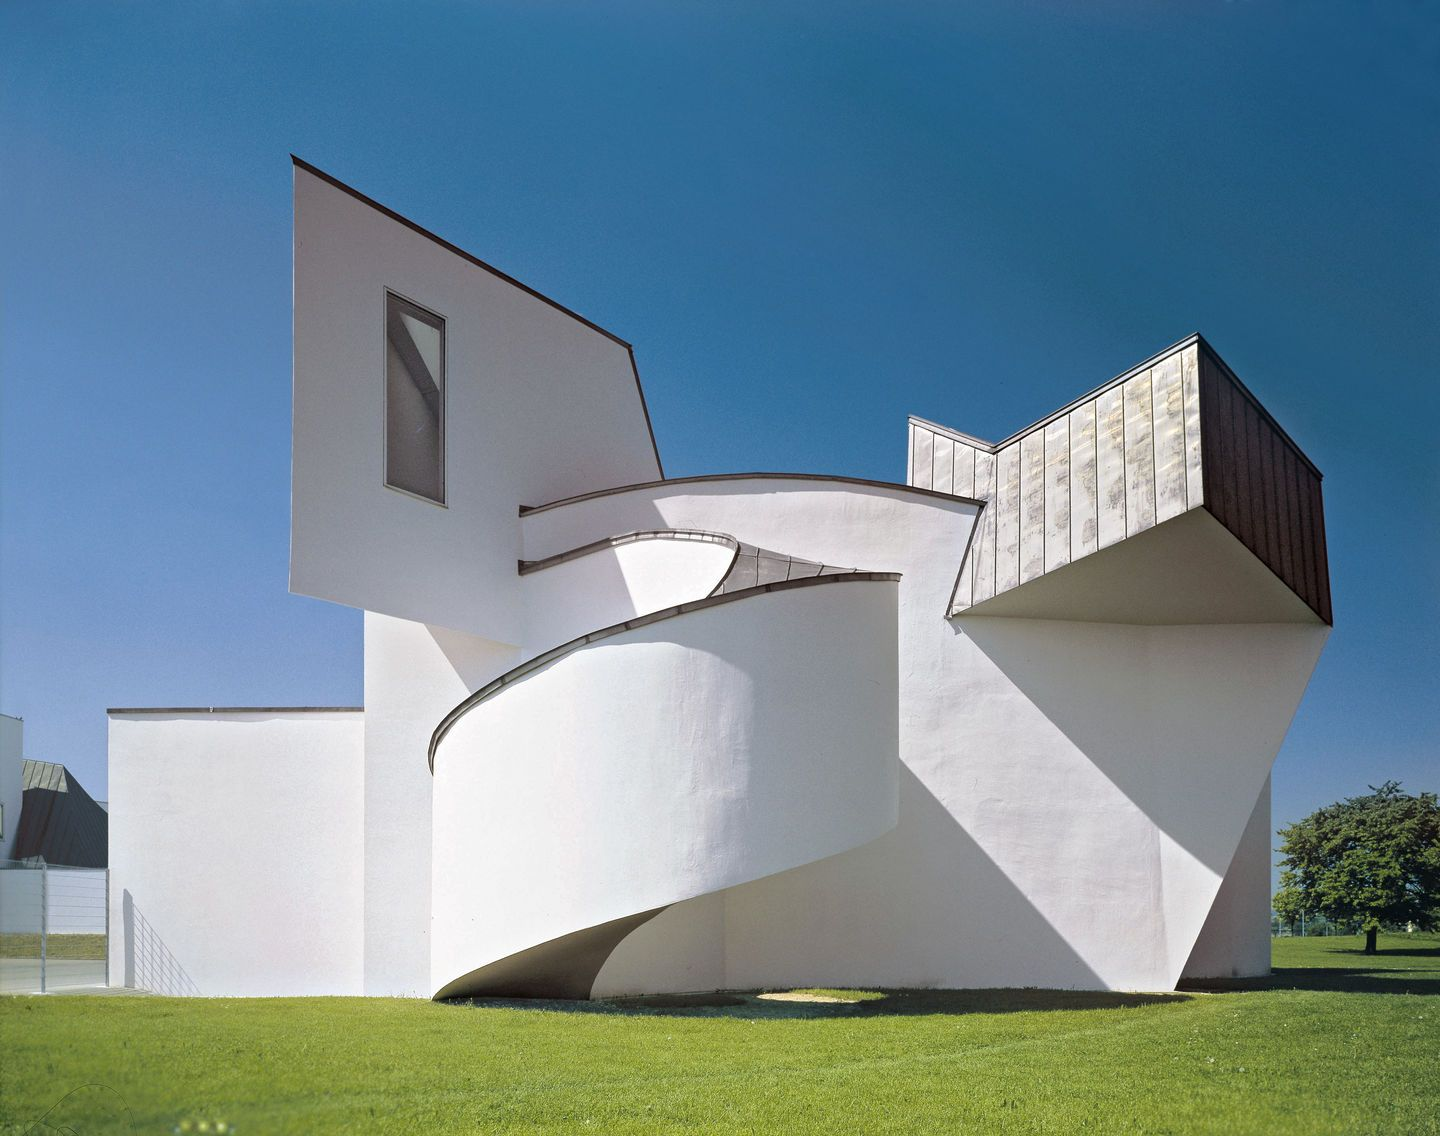
\includegraphics[height=0.6\paperheight]{images/vitra.jpg}
\end{center}
\end{frame}
\begin{frame}
\begin{center}
\Large
8. This is the opening verse to which song?
\begin{center}
    \begin{minipage}{0.6\textwidth}
        \textit{%
            Some boys kiss me \\
            Some boys hug me \\
            I think they're ok \\
            If they don't give me proper credit \\
            I just walk away}%
    \end{minipage}
\end{center}

\end{center}
\end{frame}
\begin{frame}
\begin{center}
\Huge
Answers
\end{center}
\end{frame}
\begin{frame}
\begin{center}
\Large
1. What was the nationality of the first European explorer to discover New Zealand?
\\
\onslide<2->{\vspace{1em}\textit{Dutch}}
\end{center}
\end{frame}
\begin{frame}
\begin{center}
\Large
2. the Pritzker Prize is the most prestigious international prize in what field?
\\
\onslide<2->{\vspace{1em}\textit{Architecture}}
\end{center}
\end{frame}
\begin{frame}
\begin{center}
\Large
3. ``Prophet Song'', ``The Seven Moons of Maali Almeida'', and ``The Promise'' are all prize-winning whats?
\\
\onslide<2->{\vspace{1em}\textit{Novels -- in fact, they are the three most recent Booker Prize winners}}
\end{center}
\end{frame}
\begin{frame}
\begin{center}
\Large
4. gaberdine, lawn, brocade, and french terry are all examples of what?
\\
\onslide<2->{\vspace{1em}\textit{fabrics}}
\end{center}
\end{frame}
\begin{frame}
\begin{center}
\Large
5. In 2023, researchers discovered that the T-Rex had what body part? Its presence would make them appear much less scary.
\\
\onslide<2->{\vspace{1em}\textit{lips}}
\end{center}
\end{frame}
\begin{frame}
\begin{center}
\Large
6. In the context of philosphy, what is ``Materialism''
\\
\onslide<2->{\vspace{1em}\textit{The theory in which physical matter is the only reality and that all being, processes, and phenomena can be explained as manifestations or results of matter}}
\end{center}
\end{frame}
\begin{frame}
\begin{center}
\Large
7. What is this famous building?
\\
\vspace{0.5em}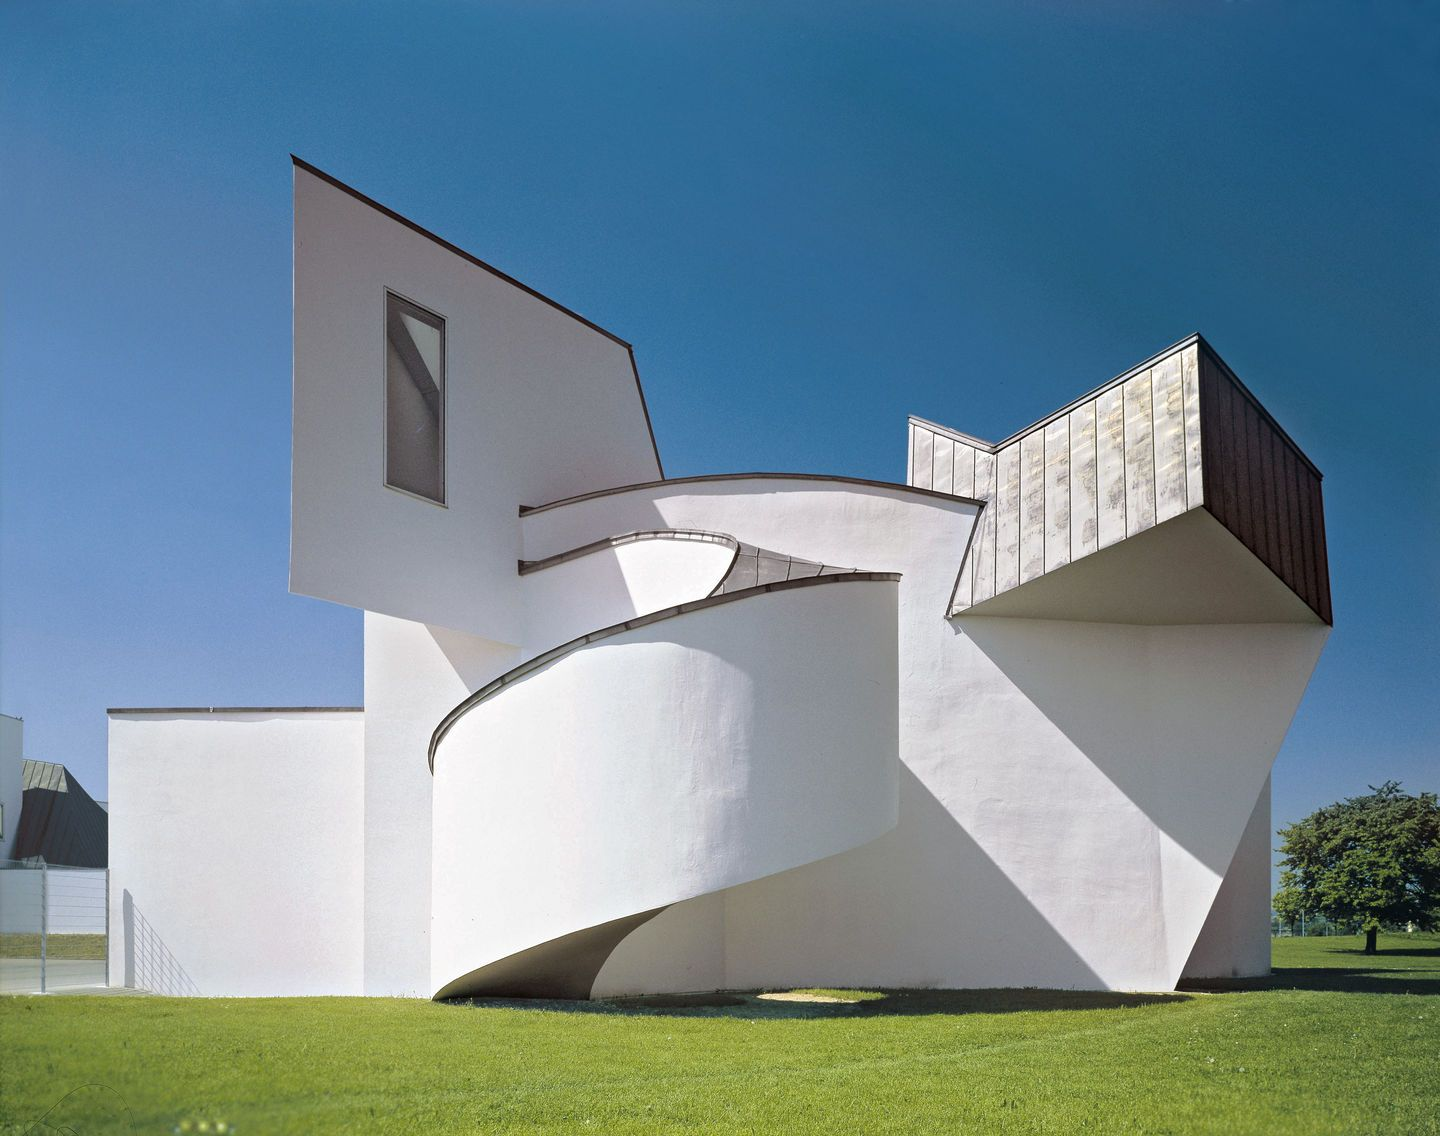
\includegraphics[height=0.6\paperheight]{images/vitra.jpg}
\\
\onslide<2->{\vspace{1em}\textit{Vitra Design Museum (Basel)}}
\end{center}
\end{frame}
\begin{frame}
\begin{center}
\Large
8. This is the opening verse to which song?
\begin{center}
    \begin{minipage}{0.6\textwidth}
        \textit{%
            Some boys kiss me \\
            Some boys hug me \\
            I think they're ok \\
            If they don't give me proper credit \\
            I just walk away}%
    \end{minipage}
\end{center}

\onslide<2->{\vspace{1em}\textit{Material Girl (Madonna)}}
\end{center}
\end{frame}
\begin{frame}
\begin{center}
\Huge
Round 4: Changing things up
\end{center}
\end{frame}
\begin{frame}
\begin{center}
\Large
1. ?
\end{center}
\end{frame}
\begin{frame}
\begin{center}
\Large
2. Which 2023 TV show was ridiculed for the appearance of ghosts?
\end{center}
\end{frame}
\begin{frame}
\begin{center}
\Large
3. Film with dollar in the title e.g. Which film pipped The Aviator to best picture in 2004?
\end{center}
\end{frame}
\begin{frame}
\begin{center}
\Large
4. ?
\end{center}
\end{frame}
\begin{frame}
\begin{center}
\Large
5. What kind of dog is this?
\\
\vspace{0.5em}
\includegraphics[height=0.6\paperheight]{images/doge.jpg}
\end{center}
\end{frame}
\begin{frame}
\begin{center}
\Large
6. What major sporting tournament is being held in Germany later this year?
\end{center}
\end{frame}
\begin{frame}
\begin{center}
\Large
7. Who wrote "Atlas Shrugged"? is a novel that is very influential in libertarian and conservative circles, especially in America
\end{center}
\end{frame}
\begin{frame}
\begin{center}
\Large
8. What links the answers to all the questions in this round?
\end{center}
\end{frame}
\begin{frame}
\begin{center}
\Huge
Answers
\end{center}
\end{frame}
\begin{frame}
\begin{center}
\Large
1. ?
\\
\onslide<2->{\vspace{1em}\textit{Franc someone? (Francis Drake)}}
\end{center}
\end{frame}
\begin{frame}
\begin{center}
\Large
2. Which 2023 TV show was ridiculed for the appearance of ghosts?
\\
\onslide<2->{\vspace{1em}\textit{The Crown}}
\end{center}
\end{frame}
\begin{frame}
\begin{center}
\Large
3. Film with dollar in the title e.g. Which film pipped The Aviator to best picture in 2004?
\\
\onslide<2->{\vspace{1em}\textit{Million Dollar Baby -- not a great question}}
\end{center}
\end{frame}
\begin{frame}
\begin{center}
\Large
4. ?
\\
\onslide<2->{\vspace{1em}\textit{Centurion}}
\end{center}
\end{frame}
\begin{frame}
\begin{center}
\Large
5. What kind of dog is this?
\\
\vspace{0.5em}
\includegraphics[height=0.6\paperheight]{images/doge.jpg}
\\
\onslide<2->{\vspace{1em}\textit{a Shiba Inu}}
\end{center}
\end{frame}
\begin{frame}
\begin{center}
\Large
6. What major sporting tournament is being held in Germany later this year?
\\
\onslide<2->{\vspace{1em}\textit{The Euros}}
\end{center}
\end{frame}
\begin{frame}
\begin{center}
\Large
7. Who wrote "Atlas Shrugged"? is a novel that is very influential in libertarian and conservative circles, especially in America
\\
\onslide<2->{\vspace{1em}\textit{Ayn Rand}}
\end{center}
\end{frame}
\begin{frame}
\begin{center}
\Large
8. What links the answers to all the questions in this round?
\\
\onslide<2->{\vspace{1em}\textit{currencies}}
\end{center}
\end{frame}
\begin{frame}
\begin{center}
\Huge
Round 5: 10 years and counting...
\end{center}
\end{frame}
\begin{frame}
\begin{center}
\Large
1. Which element was the first to be discovered in modern times (first element discovered in modern times (i.e. excluding gold, silver, copper, iron, lead, tin, mercury, carbon, and sulfur)
\end{center}
\end{frame}
\begin{frame}
\begin{center}
\Huge
Answers
\end{center}
\end{frame}
\begin{frame}
\begin{center}
\Large
1. Which element was the first to be discovered in modern times (first element discovered in modern times (i.e. excluding gold, silver, copper, iron, lead, tin, mercury, carbon, and sulfur)
\\
\onslide<2->{\vspace{1em}\textit{phosphorus}}
\end{center}
\end{frame}
\begin{frame}
\begin{center}
\Huge
Round 6: Numbers
\end{center}
\end{frame}
\begin{frame}
\begin{center}
\Large
1. ?
\end{center}
\end{frame}
\begin{frame}
\begin{center}
\Large
2. ?
\end{center}
\end{frame}
\begin{frame}
\begin{center}
\Large
3. ?
\end{center}
\end{frame}
\begin{frame}
\begin{center}
\Large
4. How many many Pirates of the Caribbean films are there?
\end{center}
\end{frame}
\begin{frame}
\begin{center}
\Large
5. ?
\end{center}
\end{frame}
\begin{frame}
\begin{center}
\Large
6. ?
\end{center}
\end{frame}
\begin{frame}
\begin{center}
\Large
7. ?
\end{center}
\end{frame}
\begin{frame}
\begin{center}
\Large
8. ?
\end{center}
\end{frame}
\begin{frame}
\begin{center}
\Huge
Answers
\end{center}
\end{frame}
\begin{frame}
\begin{center}
\Large
1. ?
\\
\onslide<2->{\vspace{1em}\textit{7}}
\end{center}
\end{frame}
\begin{frame}
\begin{center}
\Large
2. ?
\\
\onslide<2->{\vspace{1em}\textit{6}}
\end{center}
\end{frame}
\begin{frame}
\begin{center}
\Large
3. ?
\\
\onslide<2->{\vspace{1em}\textit{3}}
\end{center}
\end{frame}
\begin{frame}
\begin{center}
\Large
4. How many many Pirates of the Caribbean films are there?
\\
\onslide<2->{\vspace{1em}\textit{5}}
\end{center}
\end{frame}
\begin{frame}
\begin{center}
\Large
5. ?
\\
\onslide<2->{\vspace{1em}\textit{4}}
\end{center}
\end{frame}
\begin{frame}
\begin{center}
\Large
6. ?
\\
\onslide<2->{\vspace{1em}\textit{2}}
\end{center}
\end{frame}
\begin{frame}
\begin{center}
\Large
7. ?
\\
\onslide<2->{\vspace{1em}\textit{1}}
\end{center}
\end{frame}
\begin{frame}
\begin{center}
\Large
8. ?
\\
\onslide<2->{\vspace{1em}\textit{8}}
\end{center}
\end{frame}
\begin{frame}
\begin{center}
\Huge
Pictures: Sizing up the world
\end{center}
\end{frame}
\begin{frame}
\begin{center}
\Large
1. 
\\
\vspace{0.5em}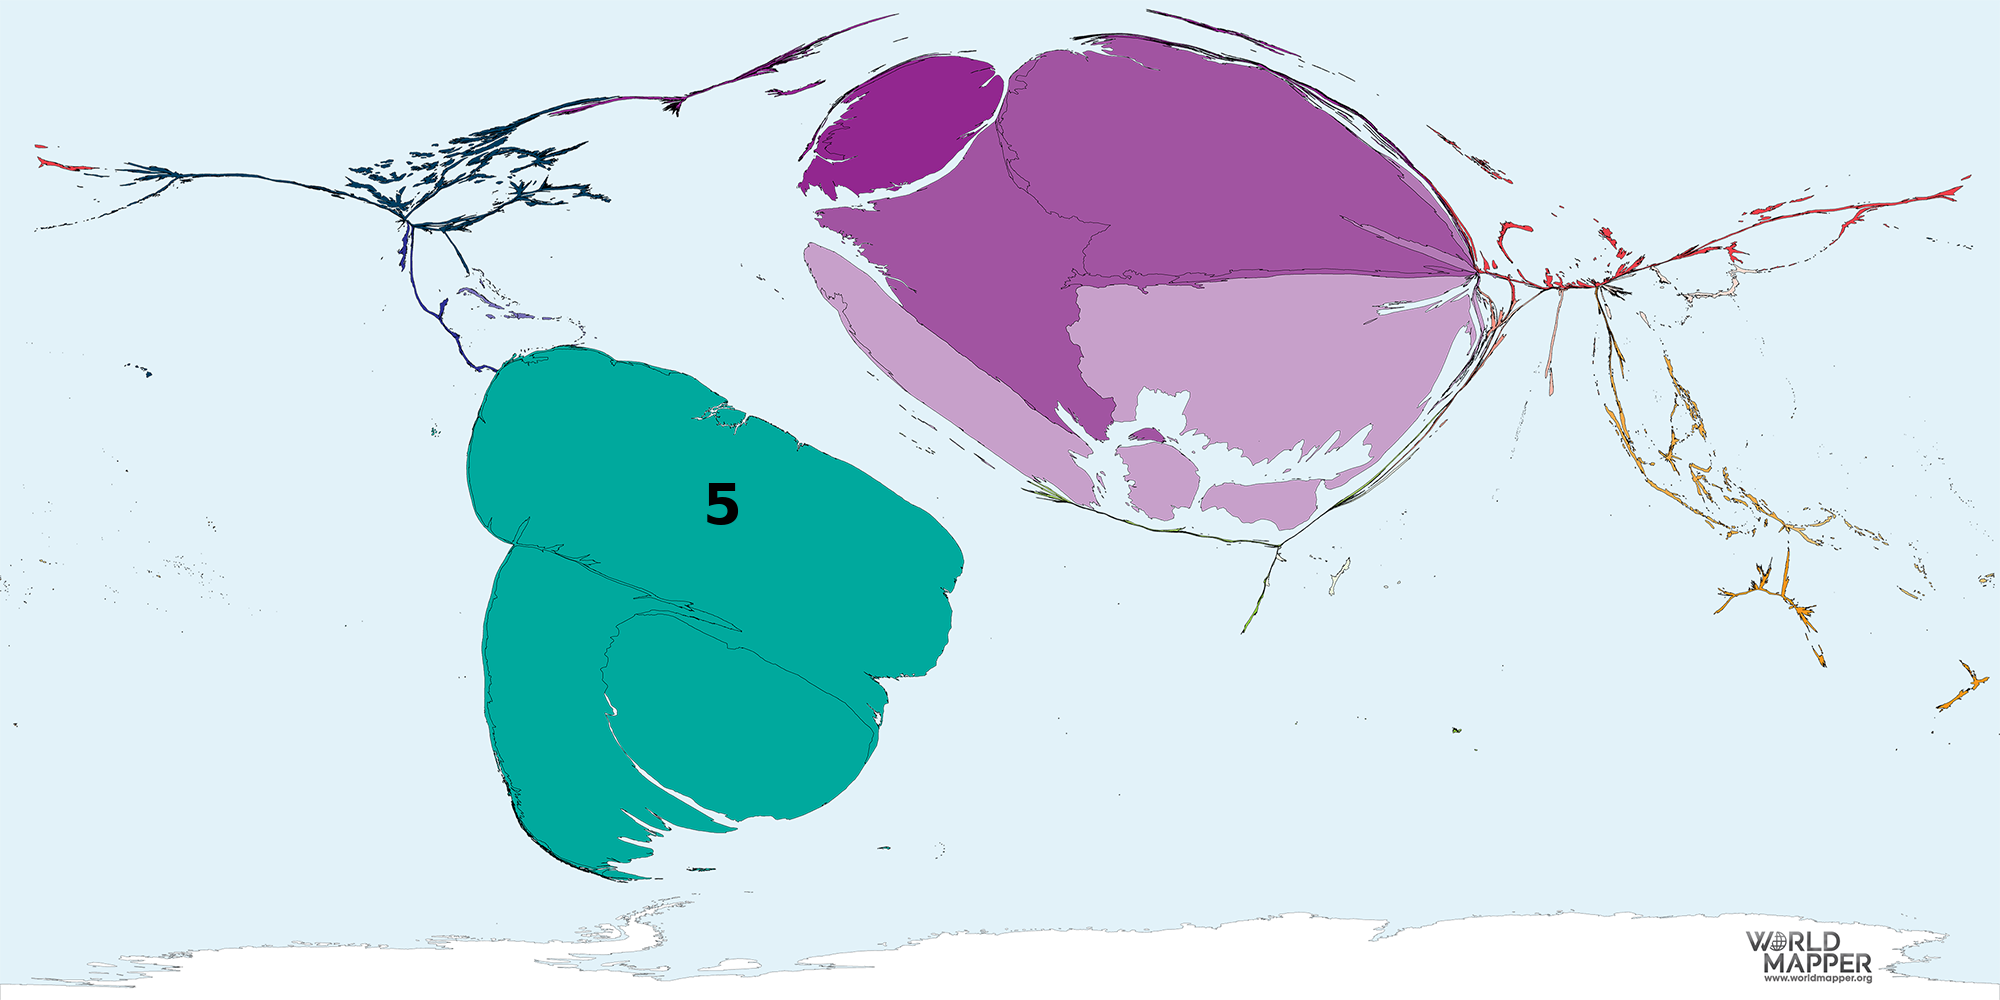
\includegraphics[height=0.6\paperheight]{maps/picture_1.png}
\\
\onslide<2->{\vspace{1em}\textit{GDP (purchasing-parity-power-adjusted)}}
\end{center}
\end{frame}
\begin{frame}
\begin{center}
\Large
2. 
\\
\vspace{0.5em}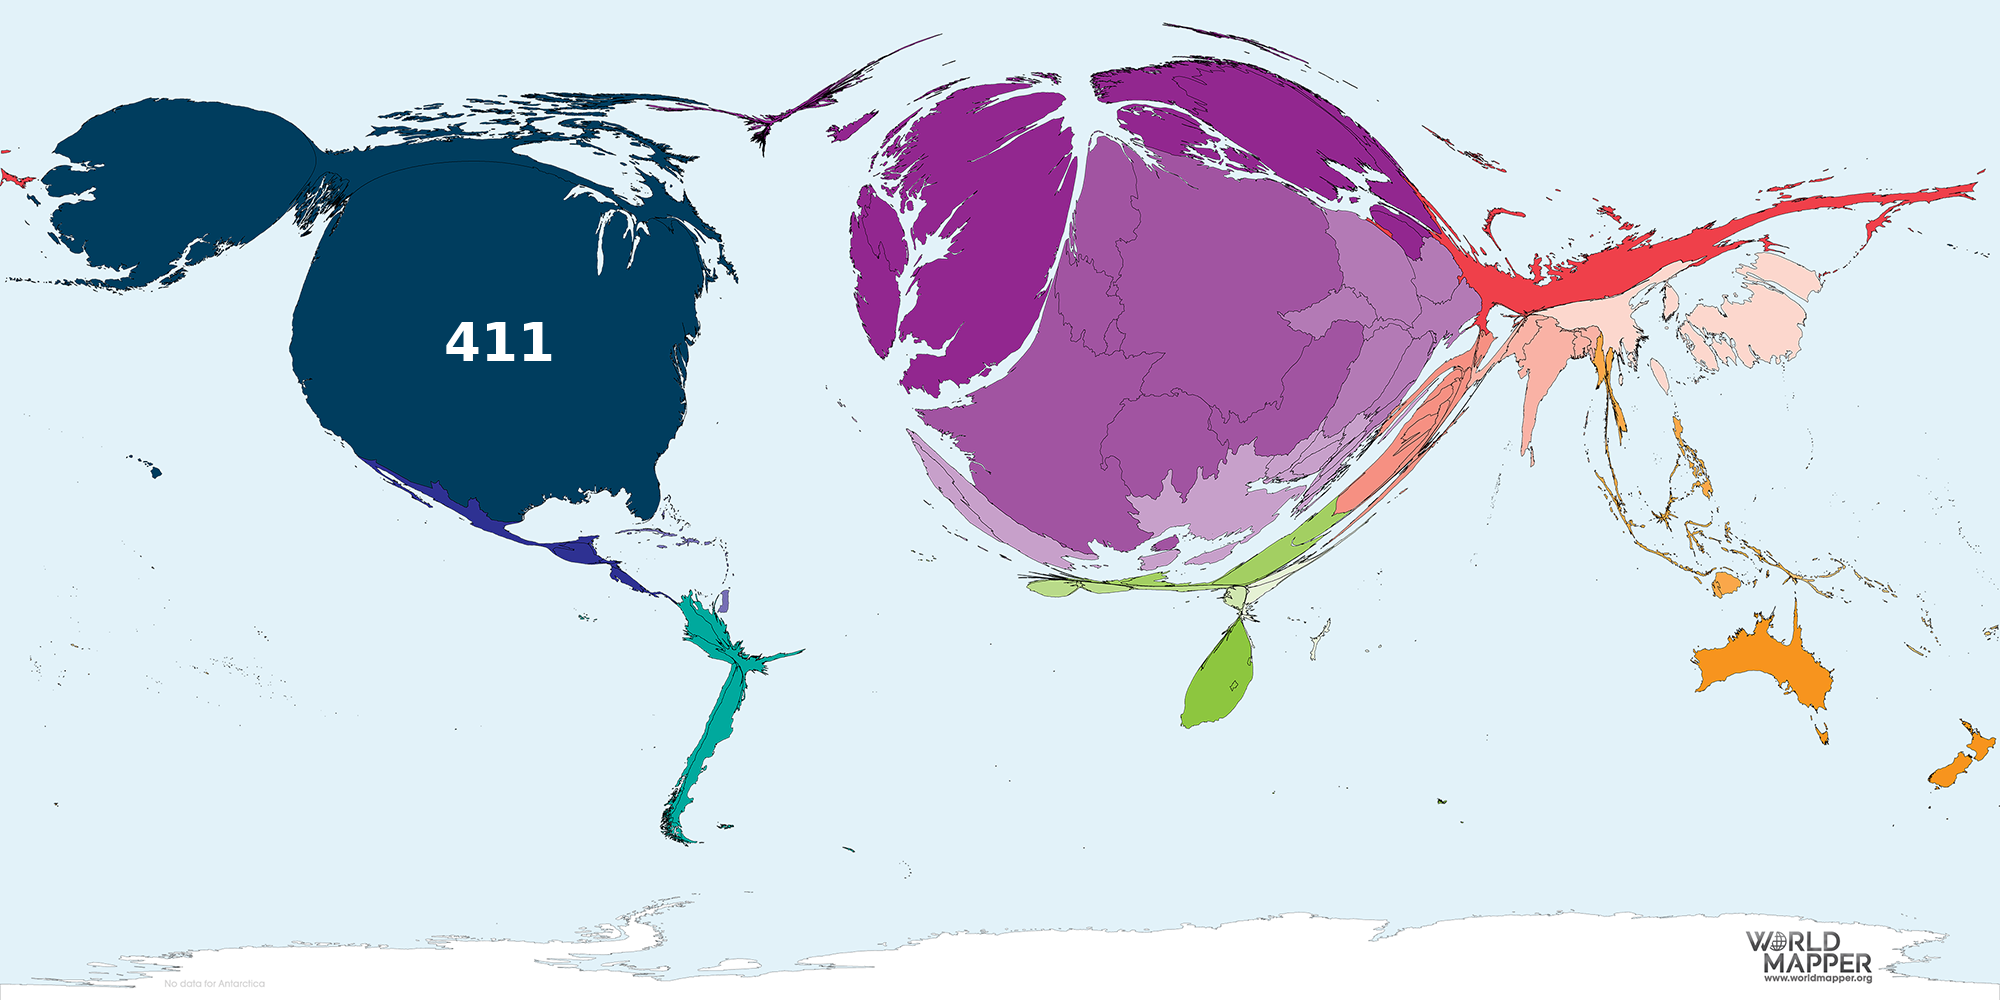
\includegraphics[height=0.6\paperheight]{maps/picture_2.png}
\\
\onslide<2->{\vspace{1em}\textit{Nobel laureates}}
\end{center}
\end{frame}
\begin{frame}
\begin{center}
\Large
3. 
\\
\vspace{0.5em}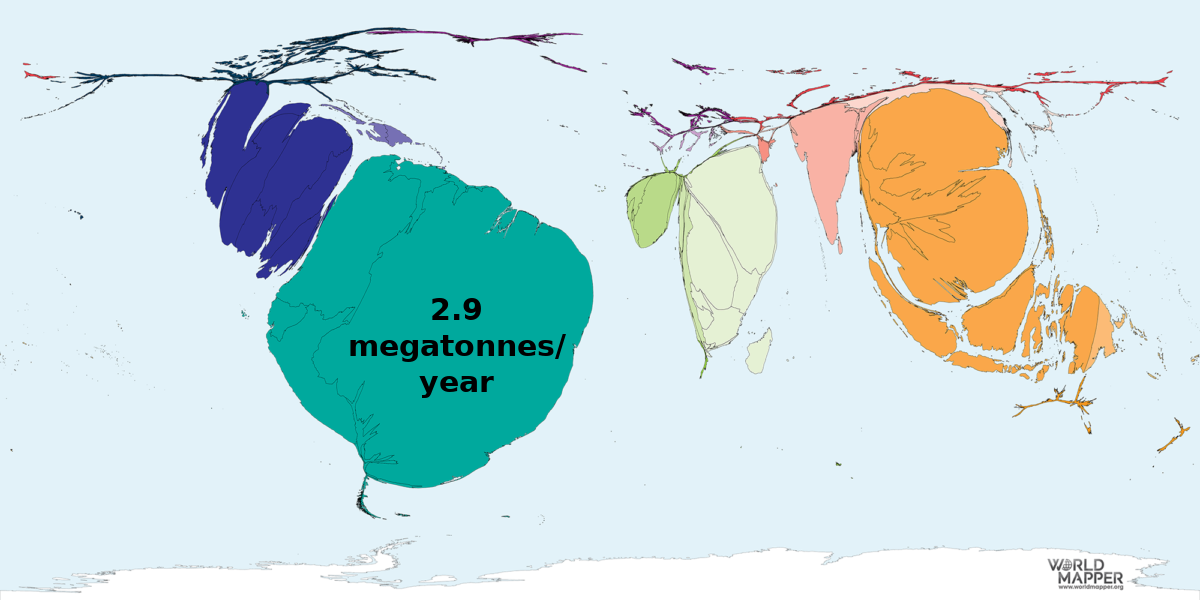
\includegraphics[height=0.6\paperheight]{maps/picture_3.png}
\\
\onslide<2->{\vspace{1em}\textit{coffee production}}
\end{center}
\end{frame}
\begin{frame}
\begin{center}
\Large
4. 
\\
\vspace{0.5em}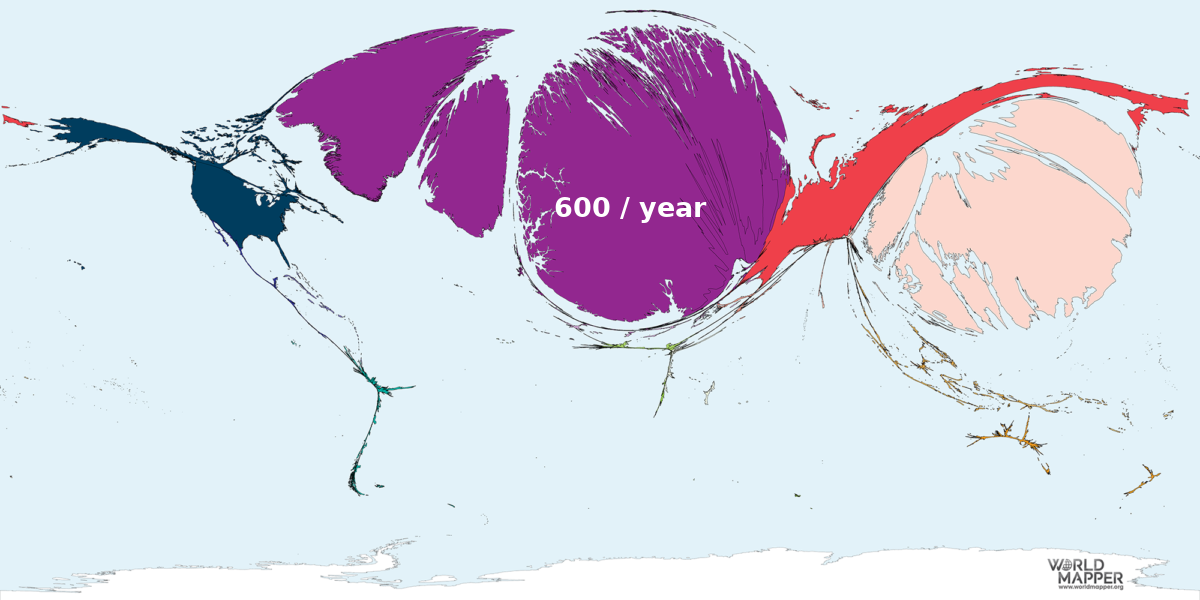
\includegraphics[height=0.6\paperheight]{maps/picture_4.png}
\\
\onslide<2->{\vspace{1em}\textit{whales killed}}
\end{center}
\end{frame}
\begin{frame}
\begin{center}
\Large
5. 
\\
\vspace{0.5em}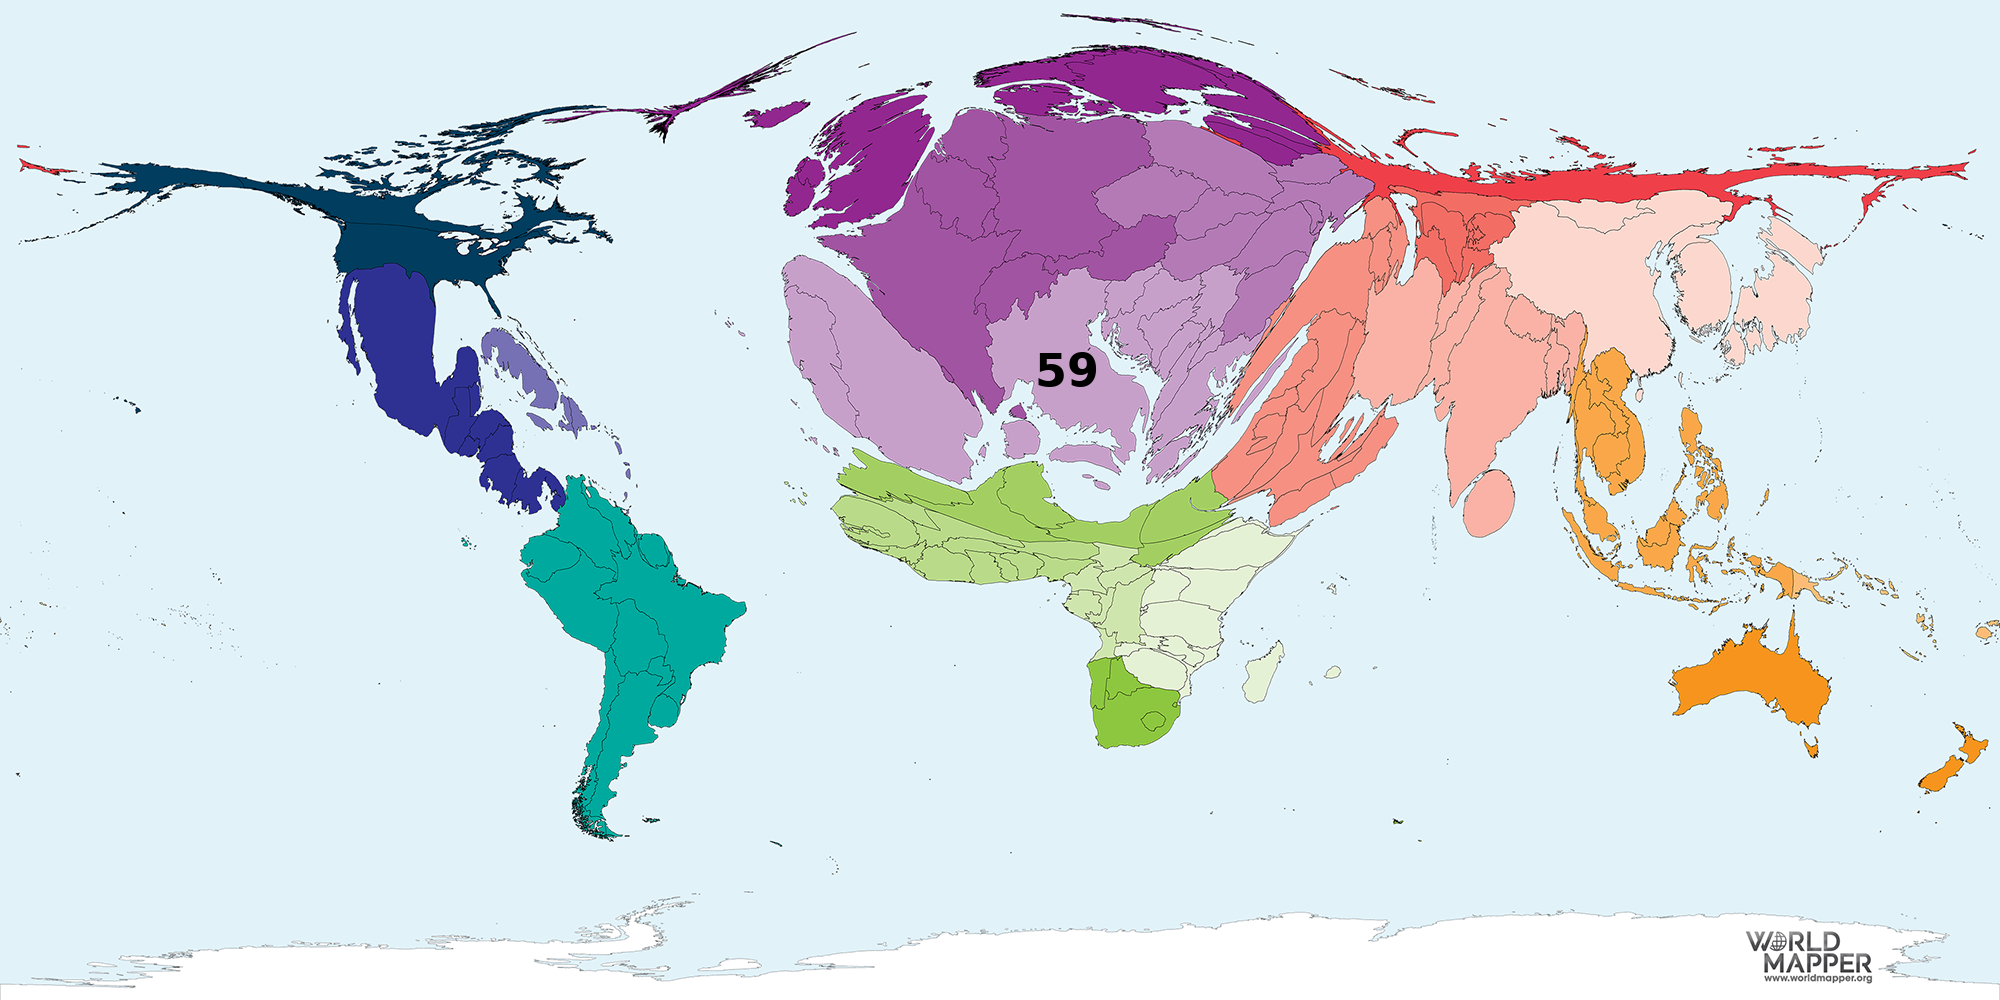
\includegraphics[height=0.6\paperheight]{maps/picture_5.png}
\\
\onslide<2->{\vspace{1em}\textit{population}}
\end{center}
\end{frame}
\begin{frame}
\begin{center}
\Large
6. 
\\
\vspace{0.5em}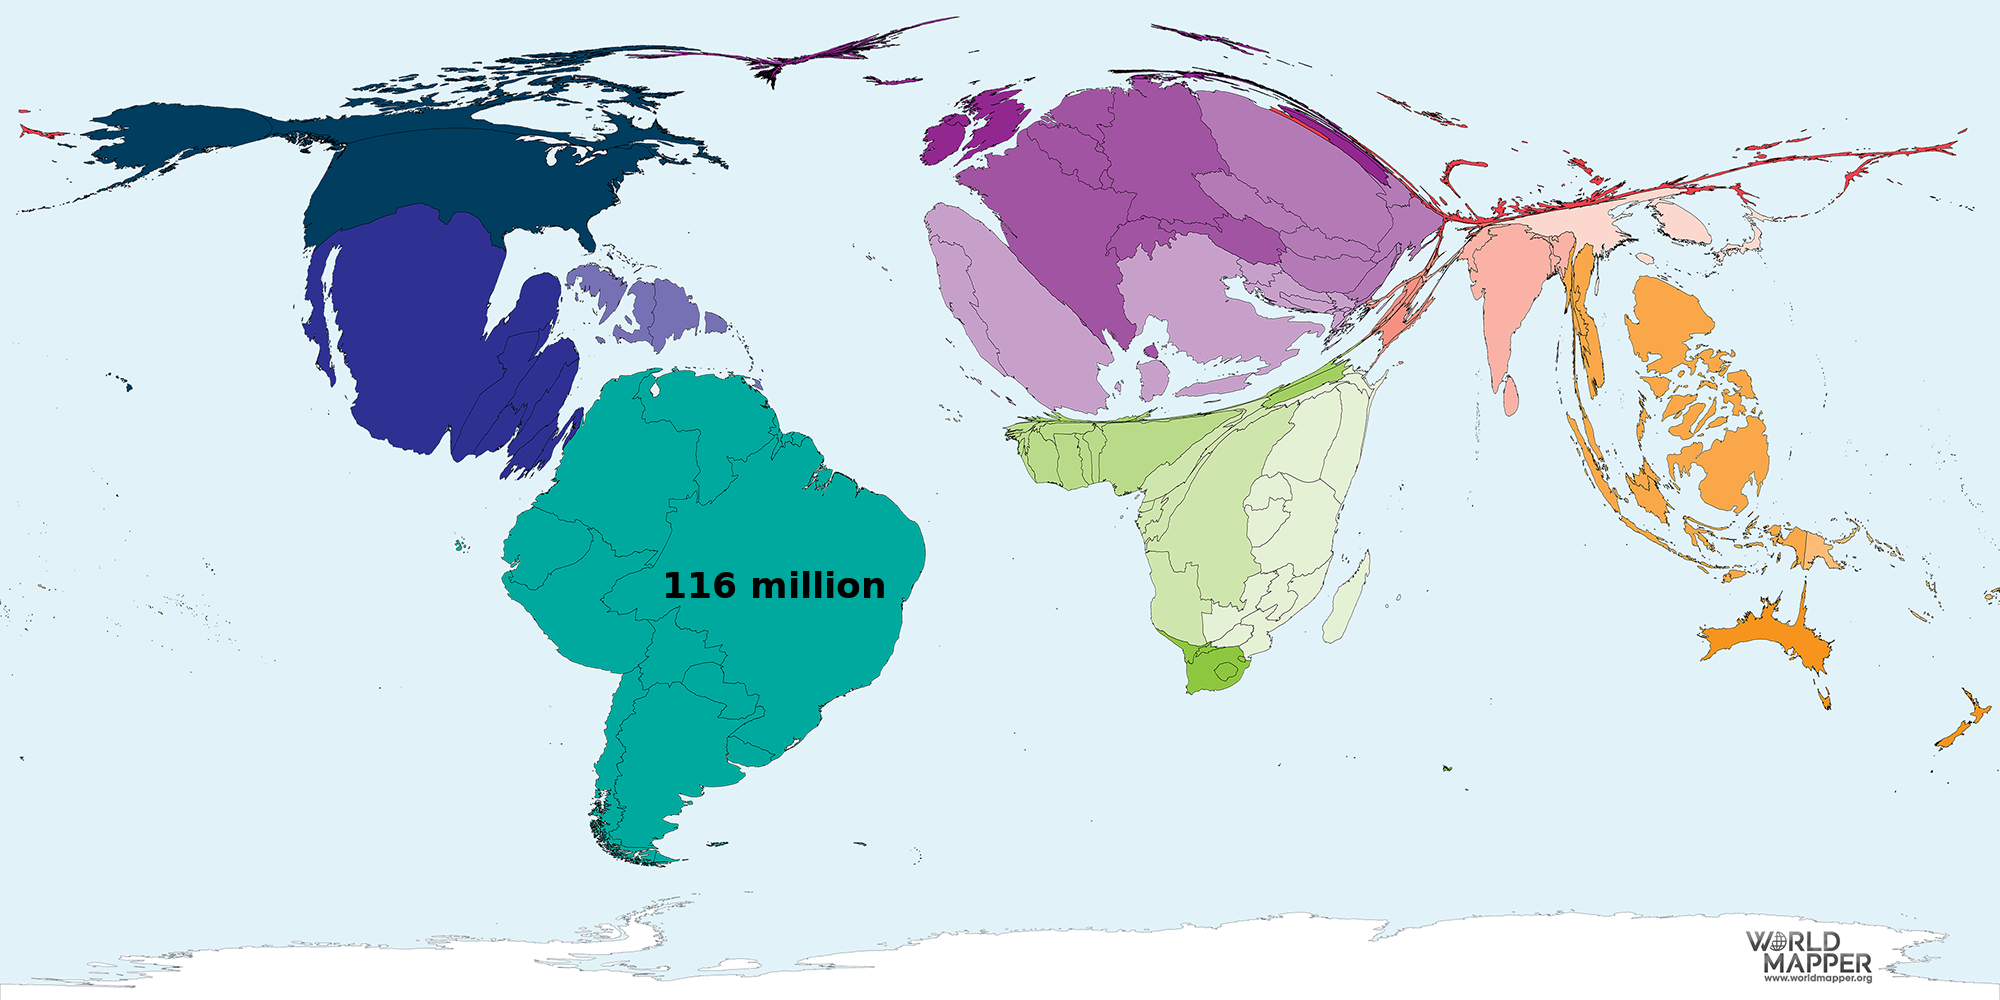
\includegraphics[height=0.6\paperheight]{maps/picture_6.png}
\\
\onslide<2->{\vspace{1em}\textit{number of Catholics}}
\end{center}
\end{frame}
\begin{frame}
\begin{center}
\Large
7. 
\\
\vspace{0.5em}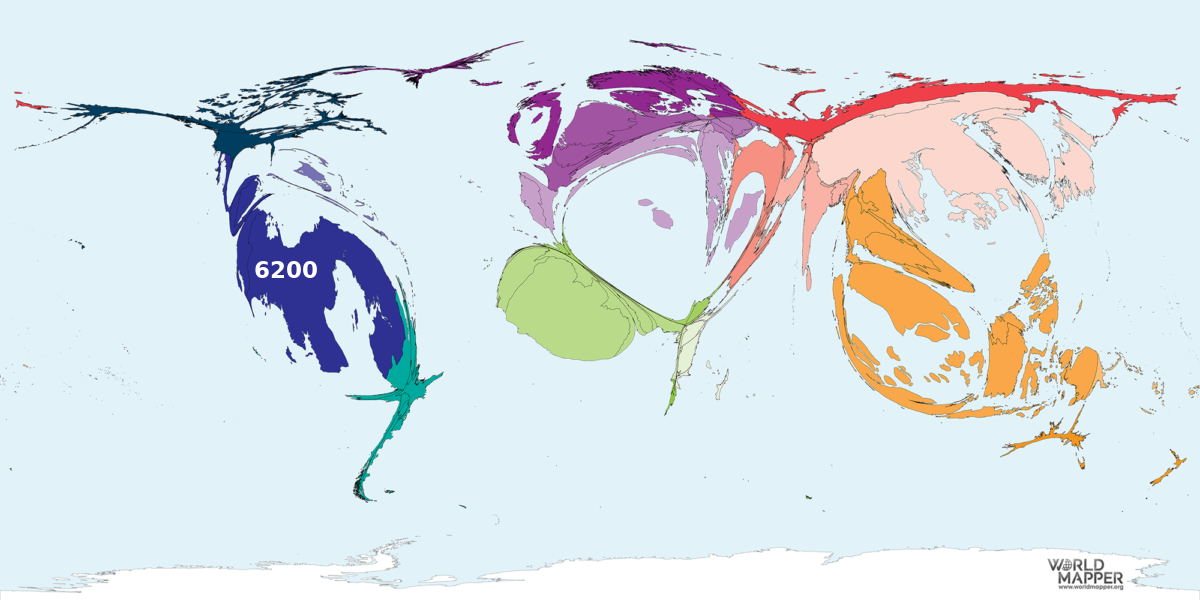
\includegraphics[height=0.6\paperheight]{maps/picture_7.png}
\\
\onslide<2->{\vspace{1em}\textit{number of registered ships}}
\end{center}
\end{frame}
\begin{frame}
\begin{center}
\Large
8. 
\\
\vspace{0.5em}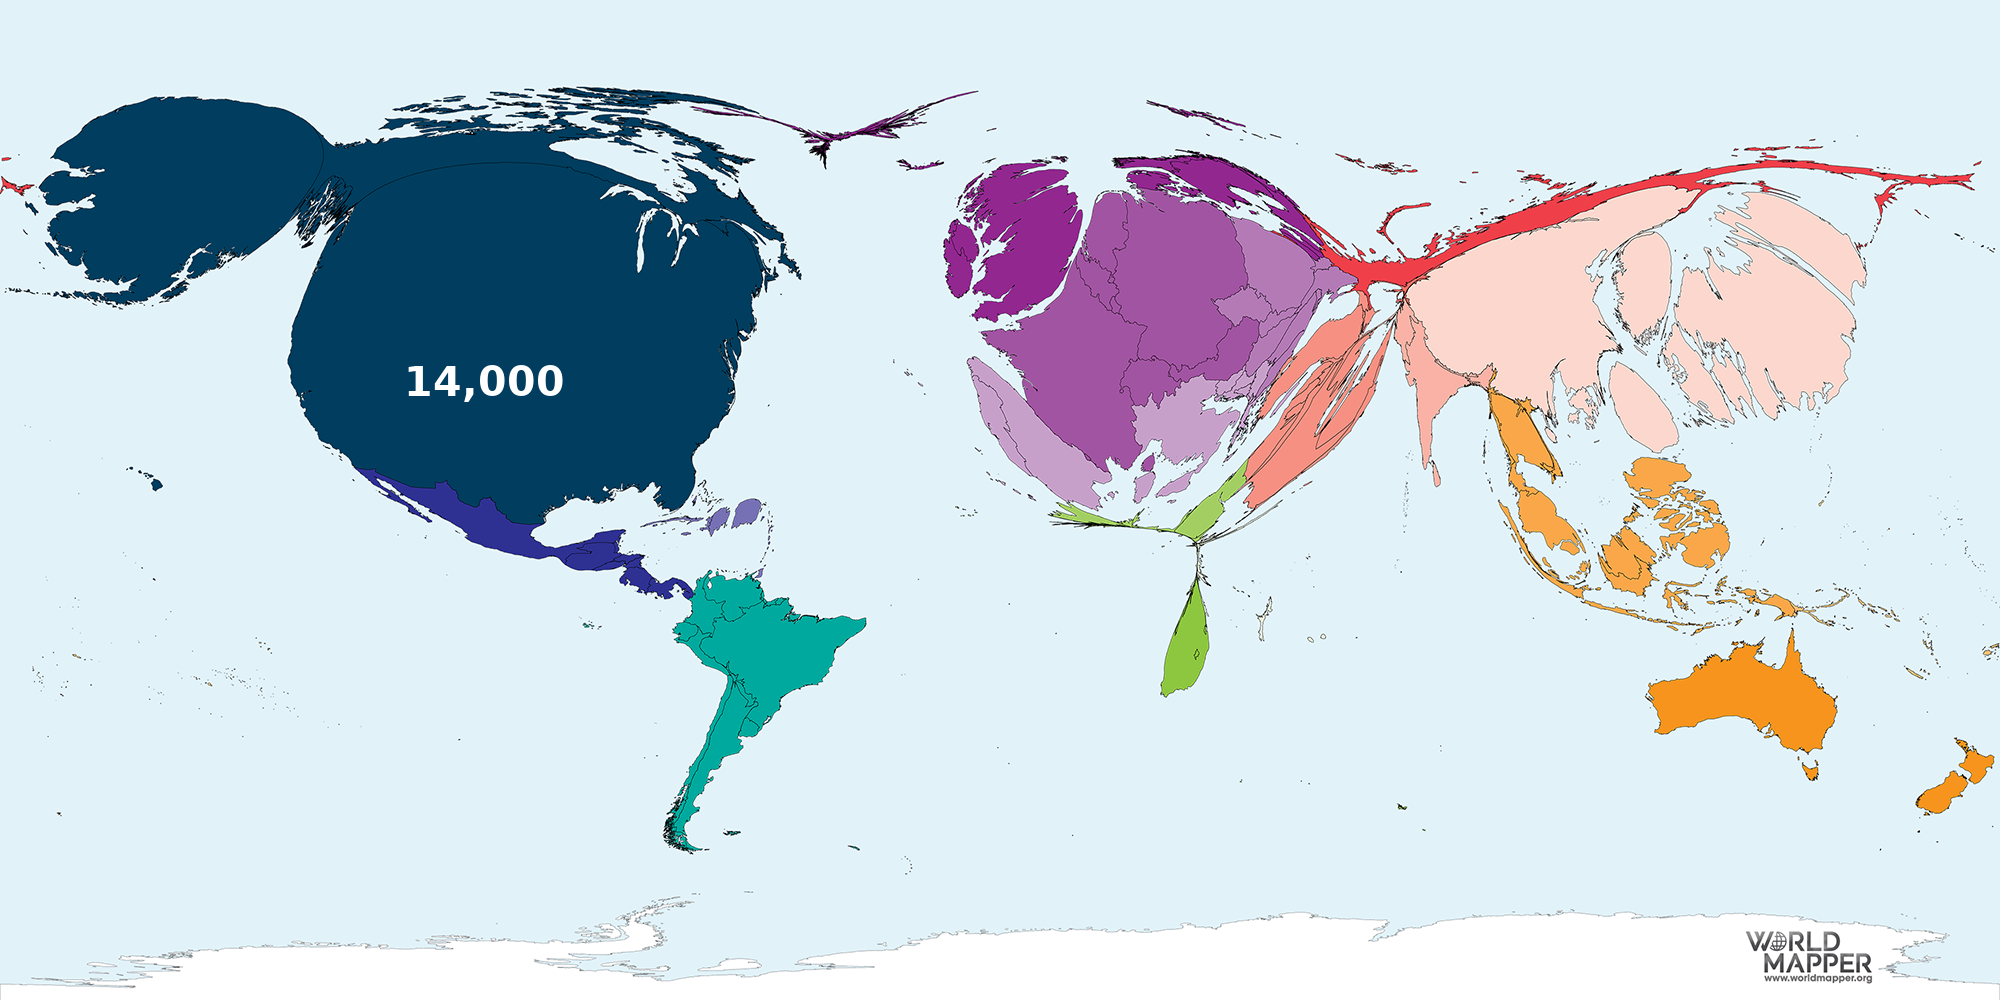
\includegraphics[height=0.6\paperheight]{maps/picture_8.png}
\\
\onslide<2->{\vspace{1em}\textit{number of McDonalds}}
\end{center}
\end{frame}
\begin{frame}
\begin{center}
\Huge
Puzzles: Connect Four
\end{center}
\end{frame}
\begin{frame}
\begin{center}
\Large
1. \leavevmode \\
\begin{center}
    \begin{minipage}{0.6\textwidth}
        \textit{%
            sharp taste \\
            words set to music \\
            Solo character \\
            archenemy of Flash Gordon}%
    \end{minipage}
\end{center}

\onslide<2->{\vspace{1em}\textit{Tang, Song, Han, and Ming: all Chinese dynasties}}
\end{center}
\end{frame}
\begin{frame}
\begin{center}
\Large
2. \leavevmode \\
\begin{center}
\setchessboard{boardfontsize=8pt, labelleft=false, labelbottom=false} % , labelfontsize=6pt
\newgame
\chessboard[setfen=4K3/8/8/8/8/8/8/8 w - - 0 0,showmover=False]
\chessboard[setfen=8/8/6K1/8/8/8/8/8 w - - 0 0,showmover=False]
\chessboard[setfen=8/8/8/8/8/8/4Q3/8 w - - 0 0,showmover=False]
\chessboard[setfen=8/8/8/8/8/2K5/8/8 w - - 0 0,showmover=False]
\end{center}
\onslide<2->{\vspace{1em}\textit{Ke8, Kg6, Qe2, and Kc3: British monarchs (Edward VIII, George VI, Elizabeth II, and Charles III)}}
\end{center}
\end{frame}
\begin{frame}
\begin{center}
\Large
3. \leavevmode \\
\begin{center}
    \begin{minipage}{0.6\textwidth}
        \textit{%
            a pew, Mr. Cuban, is a standard \\
            an entrance room, Mr. Cavendish, is a cheesy movie \\
            a profession, Mr. Twain, is a type of intellectual property \\
            a country, Mr. Hamill, is a monument}%
    \end{minipage}
\end{center}

\onslide<2->{\vspace{1em}\textit{benchmark, hallmark, trademark, and landmark}}
\end{center}
\end{frame}
\begin{frame}
\begin{center}
\Large
4. \leavevmode \\
\begin{center}
    \begin{minipage}{0.6\textwidth}
        \textit{%
            Test: objection and competition \\
            Found: deep and confuse \\
            Tract: extend and agreement \\
            Duct: goods and behaviour}%
    \end{minipage}
\end{center}

\onslide<2->{\vspace{1em}\textit{pros and cons}}
\end{center}
\end{frame}
\include{picture_slides}
\end{document}